\documentclass[tikz]{standalone} 
% change to font used in beamer
%\renewcommand{\familydefault}{\sfdefault}

\usetikzlibrary{patterns}

\begin{document}
	
	%\tdplotsetmaincoords{0}{0}
	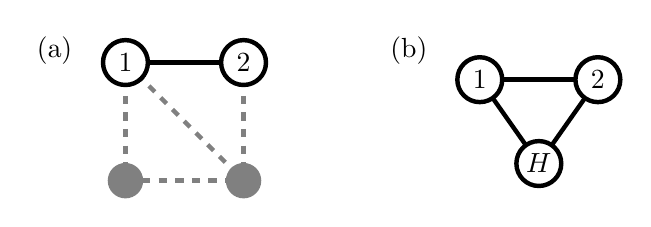
\begin{tikzpicture}[scale=1.5]
		\draw[ultra thick] (0,0) to (1,0);
		\draw[ultra thick,gray,dashed] (0,0) to (0,-1);
		\draw[ultra thick,gray,dashed] (1,0) to (1,-1);
		\draw[ultra thick,gray,dashed] (0,0) to (1,-1);
		\draw[ultra thick,gray,dashed] (0,-1) to (1,-1);
		%\draw[ultra thick,gray,dashed] (0,-1) to (0.5,-1.7);
		%\draw[ultra thick,gray,dashed] (0.5,-1.7) to (0.5,-1.7);
		%\draw[ultra thick,gray,dashed] (0.5,-1.7) to (1,-1);
		\draw[ultra thick,fill=white] (0,0) circle (0.19) node[]{$1$};
		\draw[ultra thick,fill = white] (1,0) circle (0.19) node[]{$2$};
		\fill[gray] (0,-1) circle (0.15);
		\fill[gray] (1,-1) circle (0.15);
		%\fill[gray] (0.5,-1.7) circle (0.15);
		
		\begin{scope}[shift={(3,-0.145)}]
			\draw[] (-0.6,0.245) node[]{(b)};
			\draw[ultra thick] (0,0) to (1,0);
			\draw[ultra thick] (0,0) to (0.5,-0.71);
			\draw[ultra thick] (1,0) to (0.5,-0.71);
			\draw[ultra thick,fill=white] (0,0) circle (0.19) node[]{$1$};
			\draw[ultra thick,fill = white] (1,0) circle (0.19) node[]{$2$};
			\draw[ultra thick,fill=white] (0.5,-0.71) circle (0.19) node[]{$H$};
		\end{scope}
		
		\draw[] (-0.6,0.1) node[]{(a)};
	\end{tikzpicture}
	
\end{document}